\documentclass[usenames,dvipsnames, 9pt, aspectratio=169]{beamer}
\usepackage{amsmath,amsfonts,amssymb}
\usepackage{mathtools}
\usepackage{etex} %for Windows
\usepackage[utf8]{inputenc}
\usepackage[english]{babel} 
%\usepackage[russian]{babel}
%\usepackage{microtype}			% Better interword spacing and additional kerning.
\usepackage{ellipsis}			% Adjusted space with \dots between two words.
\usepackage{graphicx}
\usepackage{pstricks}

\usepackage{xcolor}


\usepackage{changepage}

\usepackage{algorithm}
\usepackage{algpseudocode}
%\usepackage[]{algorithm2e}
%\usepackage{algorithmic}





\usepackage{tikz}
\usetikzlibrary{tikzmark,calc}
\usetikzlibrary{positioning, backgrounds}
\usetikzlibrary{arrows, chains, matrix, scopes, patterns, shapes, fit}
\usetikzlibrary{mindmap,trees,shadows}
\usetikzlibrary{decorations.pathreplacing}

\usepackage{pgfplots}



\tikzset{
	invisible/.style={opacity=0},
	visible on/.style={alt={#1{}{invisible}}},
	alt/.code args={<#1>#2#3}{%
		\alt<#1>{\pgfkeysalso{#2}}{\pgfkeysalso{#3}} % \pgfkeysalso doesn't change the path
	},
}

\newcommand\strikeout[2][]{%
	\begin{tabular}[b]{@{}c@{}} 
		\makebox(0,0)[cb]{{#1}} \\[-0.2\normalbaselineskip]
		\rlap{\color{Orange}\rule[0.5ex]{\widthof{#2}}{1.5pt}}#2
\end{tabular}}

\newcommand\Fontvi{\fontsize{11}{13.2}\selectfont}

\usepackage{listings} % for C++ code



\usepackage[T1]{fontenc}
%\usepackage[sfdefault,scaled=.85]{FiraSans}
%\usepackage{newtxsf}
%\usepackage[nomap]{FiraMono}


%\usepackage{enumerate}
%\usepackage{enumitem}



\usefonttheme[onlymath]{serif}
\renewcommand\sfdefault{cmbr}

\renewcommand{\bfdefault}{sb}




\definecolor{CharCoalDark}{RGB}{13, 16, 19}
\definecolor{Orange}{RGB}{255, 165,0}
\definecolor{DarkOrange}{RGB}{255, 165,0}
\definecolor{LightSalmon}{RGB}{255, 160, 122}
\definecolor{LeafGreen}{RGB}{34, 139,  34}
\definecolor{Coral}{RGB}{255, 127, 80}
\definecolor{DarkTurquoise}{RGB}{0, 206, 209}

%\newtheorem{defRus}{Определение}
%\newtheorem{thmRus}{Теорема}
%s\newtheorem{corRus}{Следствие}


\setbeamercolor{background canvas}{bg=CharCoalDark}

\setbeamerfont{title}{series=\bfseries}
\setbeamercolor{title}{fg=Orange}
\setbeamercolor{section in toc}{fg=white}
\setbeamercolor{frametitle}{fg=Orange}
\setbeamercolor{normal text}{fg=white}
%\setbeamercolor{normal text}{fontsize=12pt}
\setbeamercolor{itemize item}{fg=Orange}
\setbeamercolor{itemize item item}{fg=Orange}
\setbeamercolor{enumerate item}{fg=Orange}
\setbeamercolor{block title}{bg=DarkOrange,fg=white}
\setbeamerfont{block title}{series=\bfseries}

\setbeamertemplate{itemize item}[circle]
%\setbeamertemplate{itemize subitem}[$\checkmark$]
\setbeamertemplate{itemize subitem}{\color{Orange}\Large${\checkmark}$}

% footnote without a marker
\newcommand\blfootnote[1]{%
	\begingroup
	\renewcommand\footnoterule{}
	\renewcommand\thefootnote{}\footnote{#1}%
	\addtocounter{footnote}{-1}%
	\endgroup
}

\newcommand*{\Scale}[2][4]{\scalebox{#1}{\ensuremath{#2}}}%


\AtBeginSection[]
{
	\begin{frame}<beamer>
		\frametitle{Outline}
		\tableofcontents[currentsection]
	\end{frame}
}


\institute{\Large Technology Innovation Institute, Abu Dhabi, UAE}
\author{Elena Kirshanova \\ [10pt]
%	Technology Innovation Institute, Abu Dhabi, UAE
}

\title{SVP algorithms. BKZ}

\date{CIMPA Summer School, Rabat}


\setbeamertemplate{navigation symbols}{} %removes navigation

% proper highlightling of a code-snippet
\lstset{language=C++,
	keywordstyle=\color{magenta},
	stringstyle=\color{Goldenrod},
	commentstyle=\color{gray},
	breaklines=false,
	%morecomment=[l][\color{magenta}]{\#}
}

\setlength{\parskip}{8pt}

% ==================================================================
% Definitions for this paper
% ==================================================================
\mathchardef\hyphen="2D

\usepackage{multirow}
\usepackage{multicol} % For multiple coloumn environments
%\usepackage{stmaryrd} % For set brackets
% \setlength{\columnsep}{15pt} % Defining the coloumn seperation
% \setlength{\columnseprule}{1pt} % Place a line between coloumns
% \newcommand{\tab}{\hspace*{2em}}

%subscripts

\newcommand*\SmallTextScript[2]{{\mathchoice{\displaystyle #2}
		{\textstyle #2}%dito
		{\scalebox{#1}{\ensuremath{\scriptstyle #2}}}%
		{\scalebox{#1}{\ensuremath{\scriptscriptstyle #2}}}%
}}


% ADVERSARIES AND SUCH
\newcommand*{\poly}{\ensuremath{\mathrm{poly}}}
\newcommand*{\eps}{\ensuremath{\varepsilon}}

% GROUPS/DISTRIBUTIONS/SETS/LISTS
\newcommand{\N}{{{\mathbb N}}}
\newcommand{\Z}{{{\mathbb Z}}}
\newcommand*{\IZ}{\ensuremath{\mathbb{Z}}}
\newcommand*{\IN}{\ensuremath{\mathbb{N}}}
\newcommand*{\IQ}{\ensuremath{\mathbb{Q}}}
\newcommand{\R}{{{\mathbb R}}}
\newcommand*{\IR}{{{\mathbb R}}}
\newcommand{\Zp}{\ints_p} % Integers modulo p
\newcommand{\Zq}{\ints_q} % Integers modulo q
\newcommand{\Zn}{\ints_N} % Integers modulo N
\newcommand{\F}{\ensuremath{\mathbb{F}}}

\newcommand{\GF}{\ensuremath{\mathbb{F}_2}}
\newcommand{\GFn}{\ensuremath{\mathbb{F}^n_2}}

%%% ALGORITHMS/PROCEDURES %%%
\newcommand{\bigO}{\mathcal{O}}
\newcommand*{\OLandau}{\bigO}
\newcommand*{\WLandau}{\Omega}
\newcommand*{\xOLandau}{\widetilde{\OLandau}}
\newcommand*{\xWLandau}{\widetilde{\WLandau}}
\newcommand*{\TLandau}{\Theta}
\newcommand*{\xTLandau}{\widetilde{\TLandau}}
\newcommand{\smallo}{o} %technically, an omicron
\newcommand{\wLandau}{\omega}
\newcommand{\negl}{\mathrm{negl}}
\newcommand*\PROB\Pr 
\DeclareMathOperator*{\EXPECT}{\mathbb{E}}
\DeclareMathOperator*{\VARIANCE}{\mathbb{V}}
\DeclareMathOperator*{\LOGBIAS}{\mathbb{LB}}

% Lattices

% \newcommand{\coset}{\Lambda} % Lambda Lattice
% \newcommand{\cosetPerp}{\Lambda^{\bot}} % Lambda_Perp Lattice
% \newcommand{\gadget}{\textbf{G}} %Gaget matrix
% \newcommand{\mes}{\textbf{m}} %message vector
% \newcommand{\AMat}{\textbf{A}} %A matrices
% \newcommand{\BMat}{\textbf{B}} %B matrices
% \newcommand{\RMat}{\textbf{R}} %R matrices
% \newcommand{\HMat}{\textbf{H}} %H matrices
% \newcommand{\XMat}{\textbf{X}} %H matrices
% \newcommand{\mbar}{\bar{m}} %mBar dimension
% % \newcommand{\gauss}{\mathcal{D}} % gaussian distribution
% \newcommand{\Id}{\textbf{I}} % Identity matrix
% \newcommand{\er}{\textbf{e}} % gaussian distr. vectors
% % \newcommand{\cipher}{\textit{c}} % ciphertext
% \newcommand{\Olwe}{\mathcal{O}_{\textsf{LWE}}} %LWE oracle
% \newcommand{\OSample}{\mathcal{O}_{Sample}} %LWE oracle
% \newcommand{\SigmaB}{\boldsymbol{\Sigma}} %semi-deifinite matrix Sigma%
% % \newcommand{\mods}{\text{ mod}}


%Vectors and Matrices

\newcommand{\AMat}{\mathbf{A}} %A matrices
\newcommand{\BMat}{\mathbf{B}} %B matrices
\newcommand{\DMat}{\mathbf{D}} %Diagonal


\newcommand{\HMat}{\ensuremath{\mathbf{H}}}
\newcommand{\QMat}{\ensuremath{\mathbf{Q}}}
\newcommand{\Id}{\ensuremath{\mathbf{I}}}
\newcommand{\ZeroM}{\textbf{0}} % Zero matrix

\newcommand{\bvec}{\ensuremath{\mathbf{b}}}
\newcommand{\evec}{\ensuremath{\mathbf{e}}}
\newcommand{\svec}{\ensuremath{\mathbf{s}}}
\newcommand{\vvec}{\ensuremath{\mathbf{v}}}
\newcommand{\zvec}{\ensuremath{\mathbf{0}}}
\newcommand{\xvec}{\ensuremath{\mathbf{x}}}
\newcommand{\yvec}{\ensuremath{\mathbf{y}}}
\newcommand{\uvec}{\ensuremath{\mathbf{u}}}

\newcommand{\nth}{^{\mathrm{th}}}

\newcommand{\RepMMT}{\ensuremath{\mathcal{R}_{\protect\SmallTextScript{0.70}{\texttt{MMT}}}}}
\newcommand{\RepBJMM}{\ensuremath{\mathcal{R}_{\protect\SmallTextScript{0.70}{\texttt{BJMM}}}}}
\newcommand{\XOR}{\ensuremath{\mathtt{3XOR}}}


% % % % % \newcommand{\mb}[1]{\mathbf{#1}} % does not compile otherwise
%%% Removed by Gotti; this is just asking to screw up with packages that (properly) define \mb (mathbold)

% \newcommand{\bL}{\|\bvec_1\|} % b1 length that appears way too often
% \newcommand{\dL}{\|\dvec_1\|} % b1 length that appears way too oftend

%Norms and Scalar products

\newcommand*\abs[1]{\left\lvert#1\right\rvert}
\newcommand*\norm[1]{\left\lVert#1\right\rVert}
\newcommand*\normalabs[1]{\lvert#1\rvert} 
\newcommand*\normalnorm[1]{\lVert#1\rVert}
\newcommand*\bignorm[1]{\bigl\lVert#1\bigr\rVert}
\newcommand*\bigabs[1]{\bigl\lvert#1\bigr\rvert}
\newcommand*\Bigabs[1]{\Bigl\lvert#1\Bigr\rvert}
\newcommand*{\ScProd}[2]{\ensuremath{\langle#1\mathbin{,}#2\rangle}} %Scalar Product
% \newcommand*{\ScProd}[2]{\ensuremath{\langle#1 \:{,}\:#2\rangle}} %Scalar Product
\newcommand*{\bigScProd}[2]{\ensuremath{\bigl\langle#1\mathbin{,}#2\bigr\rangle}} %Scalar Product
\newcommand*{\BigScProd}[2]{\ensuremath{\Bigl\langle#1\mathbin{,}#2\Bigr\rangle}} %Scalar Product


%Some other math operators

\DeclareMathOperator{\Span}{Span} %span of vectors
\DeclareMathOperator{\vol}{\mathrm{vol}} %volume
\DeclareMathOperator{\LW}{LambertW} %Lambert W function
\DeclareMathOperator{\SD}{SD}
\DeclareMathOperator{\gradient}{grad}
\DeclareMathOperator{\TRACE}{Tr}
\newcommand*{\dDR}{\mathrm{d}} %de-Rham-Differential (the d in dx, dy, dz and so on)


%Lists
\renewcommand{\L}{\ensuremath{\mathcal{L}}}

\renewcommand{\P}{\ensuremath{\mathcal{P}}}

\newcommand*{\Lout}{\ensuremath{\L_{\mkern-0.5mu\protect\SmallTextScript{0.85}{\textup{out}}}}}
\newcommand*{\Sout}{\ensuremath{S_{\mkern-0.5mu\protect\SmallTextScript{0.85}{\textup{out}}}}}
\newcommand{\wt}{\ensuremath{\mathit{wt}}}


\newcommand*{\softO}{\widetilde{\bigO}}

\newcommand{\const}{\mathsf{c}} 


\newcommand{\transpose}{\mkern0.7mu^{\mathsf{ t}}}

%proper overline reduced by 1.5mu
\newcommand{\overbar}[1]{\mkern 1.5mu\overline{\mkern-1.5mu#1\mkern-1.5mu}\mkern 1.5mu}

\DeclareMathOperator{\erf}{erf} %error function
\DeclareMathOperator{\erfc}{erfc} %complementary error function
\newcommand{\Er}{\ensuremath{\mathrm{Er}}} %complementary error function


% LATTICES

\newcommand{\Lat}{\ensuremath{\mathcal{L}}}
\newcommand*{\Sphere}[1]{\ensuremath{\mathsf{S}^{#1}}}
\DeclareMathOperator{\Conf}{Conf}

%Thick line for table
\setlength{\doublerulesep}{0pt}
\newcommand{\thickline}{\hline\hline\hline}


%circled text
\newcommand*\circled[1]{\tikz[baseline=(char.base)]{
    \node[shape=circle,draw,inner sep=0.3 pt] (char) {\scriptsize #1};}}


%Fix Algorithmicx package
\def\NoNumber#1{{\def\alglinenumber##1{}\State #1}\addtocounter{ALG@line}{-1}}

%For comments
\newcommand{\GColor}{ForestGreen}  %Damiens' color
\newcommand{\EColor}{MidnightBlue} %Elena's color

\newcommand*{\E}[1]{{\color{\EColor} #1} } 
\newcommand*{\G}[1]{{\color{\GColor} #1} } 

%Proper limit with the subscript underneath
% \newcommand{\Lim}[1]{\raisebox{0.5ex}{\scalebox{0.8}{$\displaystyle \lim_{#1}\;$}}}


%TIKZ dense dotted pattern

\pgfdeclarepatternformonly{my dots}{\pgfqpoint{-1pt}{-1pt}}{\pgfqpoint{2.0pt}{2.0pt}}{\pgfqpoint{2pt}{2pt}}%
{
	\pgfpathcircle{\pgfqpoint{0pt}{0pt}}{.35pt}
	\pgfpathcircle{\pgfqpoint{1pt}{1pt}}{.35pt}
	\pgfusepath{fill}
}


\tikzset{
	master/.style={
		execute at end picture={
			\coordinate (lower right) at (current bounding box.south east);
			\coordinate (upper left) at (current bounding box.north west);
		}
	},
	slave/.style={
		execute at end picture={
			\pgfresetboundingbox
			\path  (lower right)rectangle (upper left) ;
		}
	}
} %all defs
\begin{document}
	
\begin{frame}
	\titlepage
\end{frame}



\begin{frame}{Links}
	\Large 
	\centering
	These slides are available here: 
	\vspace{7pt}
	
	
\includegraphics[width=0.4\textwidth]{qrcodeSlides}
	
	\vspace{5pt}
	\url{https://crypto-kantiana.com/elena.kirshanova/teaching/ssRabat/SVP_Rabat.pdf}
\end{frame}

\begin{frame}{Links II}
\centering
	\Large Exercises, labs are available on the webpage:
	\vspace{7pt}
	
	
\includegraphics[width=0.4\textwidth]{qrcodeWebpage}
	
	\vspace{5pt}
	\url{https://crypto-kantiana.com/elena.kirshanova/teaching/summerschoolRabat2023.html}
\end{frame}

\begin{frame}{Agenda}
\LARGE
\begin{itemize}
	\itemsep 10pt
	\item {\color{Orange} Today:} Lectures
	\item {\color{Orange} Tomorrow:} Exercises
	\item {\color{Orange} Friday:} Labs
\end{itemize}
\end{frame}

\begin{frame}{Labs}
\LARGE 
\begin{itemize}
	\itemsep 8pt
	\item For Lab1 you need to install FPyLLL \url{https://github.com/fplll/fpylll}
	\item It is available via SageMathCell and CoCalc (select a Jupyter notebook with a Sage kernel)
	%\item I will also show the G6K library \url{https://github.com/fplll/g6k} but you're not required to install it
	\item For Lab2 and Lab3 you need Sage on your machine (Lab2 is checked via automated tests)
	\item Labs can be solved in teams of {\color{Orange} max 3} people
	\item Try to install FPyLLL or play with it in CoCalc
\end{itemize}
\end{frame}

\begin{frame}{Prize}
\Huge 
\centering
The fastest team to obtain correct$^\star$ solutions/implementations gets an unforgettable prize!

\vfill
\Large  The correctness will be judged by the lecturer
\end{frame}

%\section{Definitions}

\begin{frame}{Content of the lectures}
\LARGE
\begin{enumerate}
	\setlength\itemsep{10pt}
	\item The shortest vector problem
	\item Kannan-Finke-Pohst Enumeration algorithm
	\item Sieving algorithm \\[5pt]
	\item Block Korkine-Zolotarev reduction
	\item Solving LWE with BKZ
	
\end{enumerate}

\end{frame}

\begin{frame}
Part I \\ [10pt]
\centering
\begin{LARGE}
	
	
	\color{Orange}
	\Huge The shortest vector problem
	
\end{LARGE}
\end{frame}

\begin{frame}{A lattice: definition}
	%\tikzstyle{background grid}=[draw, gray, opacity=0.0,step=10pt]
	\vspace{-20pt}\centering
	\begin{tikzpicture}%[show background grid]
	\begin{scope}
	\foreach \y in {-2,...,4}
	\foreach \x in {-2,...,3}
		\filldraw(\x*40pt+\y*10pt, 10pt*\x+20pt*\y) circle (1.7pt);
		
	\filldraw(0pt,0pt) circle (1.7pt) node[below]{ $0$};
	
	\draw[-stealth, white, thick] (0,0) -- (50pt, 30pt) node[font=\Large, below, xshift=5pt]{$\bvec_1$};
	\draw[-stealth, white, thick] (0,0) -- (40pt, 10pt) node[font=\Large, below, xshift=5pt]{$\bvec_2$};
	\end{scope}
	%\draw[CharCoalDark] (-5,-4) rectangle (6,-1.9) node[pos=.5, color=white, opacity=1,align=left] {\Large A lattice $\mathcal{L}$ -- a set of all integer linear combination of basis vectors $\{ \vec{b}_1, \ldots, \vec{b}_n\}$ \\
%Usually, $\vec{b}_i \in \Z^n.$};
	\end{tikzpicture}
	
	\Large {\color{Orange} \textbf{A lattice}}  is the set $\mathcal{L} = \{ \sum_{i\leq n} x_i \bvec_i \; : \; x_i \in \Z \}$ for some linearly independent $\bvec_i$'s. 
		
	For us, $\bvec_i \in \Z^n$ and $\mathcal{L}$ is full-rank.
\end{frame}


\begin{frame}{Short vectors in $\L$}
	\vspace{-32pt}\centering
	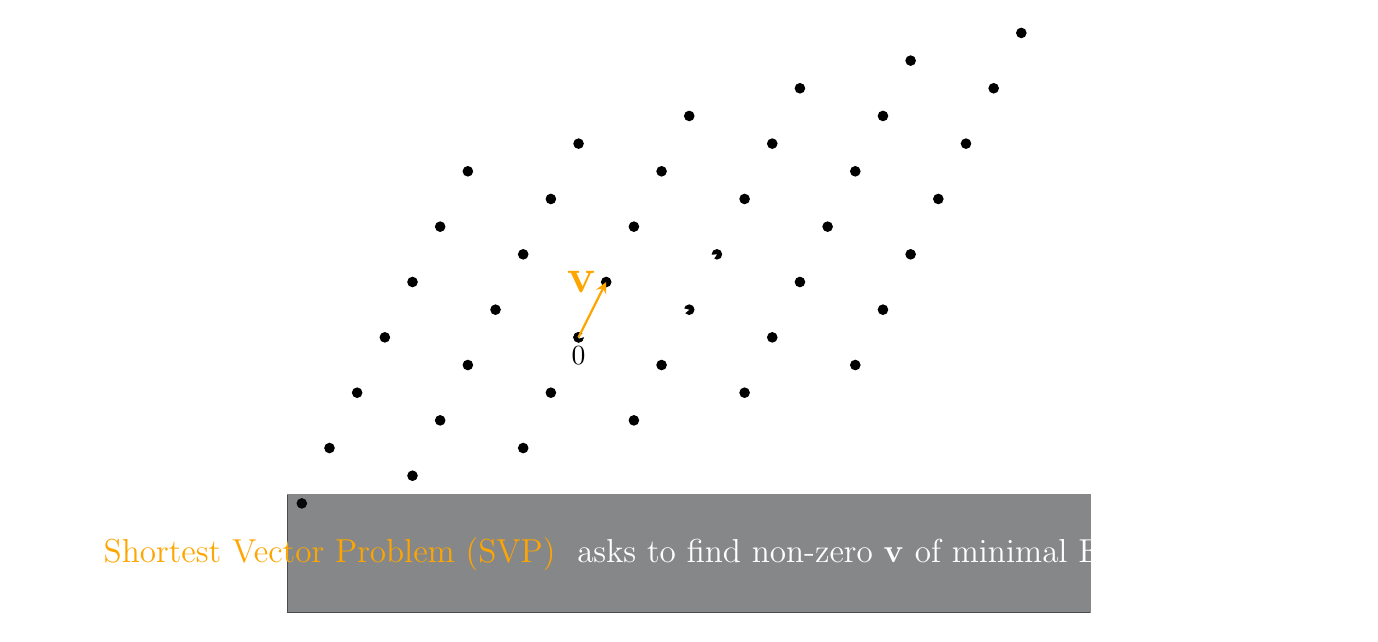
\begin{tikzpicture}%[show background grid]
	\begin{scope}
	\foreach \y in {-2,...,4}
	\foreach \x in {-2,...,3}
		\filldraw(\x*40pt+\y*10pt, 10pt*\x+20pt*\y) circle (1.7pt);	

		\filldraw(0pt,0pt) circle (1.7pt) node[below]{ $0$};

		\draw[-stealth, white, thick] (0,0) -- (50pt, 30pt) node[font=\Large, below, xshift=5pt]{$\bvec_1$};
		\draw[-stealth, white, thick] (0,0) -- (40pt, 10pt) node[font=\Large, below, xshift=5pt]{$\bvec_2$};
		
		\draw[-stealth, Orange, thick] (0, 0) -- (10pt, 20pt) node[font=\LARGE, left]{$\vvec$};
		
		\draw[fill=CharCoalDark, draw=CharCoalDark, opacity=0.5] (-3.7,-3.5) rectangle (6.5,-2.0) node[pos=.5, color=white, opacity=1,align=left] {
			\large The {\color{Orange}{Shortest Vector Problem} (SVP) } asks to find non-zero $\vvec$ of minimal Euclidean length. 
		}; 
	\end{scope}
	\end{tikzpicture}
	
	\vspace{-5pt}
	\large We do not know $||\vvec||$ in general, but for any $n$-rank $\L$:
	\[||\vvec_{\text{shortest}}|| \leq \sqrt{n} \cdot \det(\L)^{1/n}  \quad \text{(Minkowski's bound)}
	\]
\end{frame}

\begin{frame}{Hardness of SVP (small-order terms are omitted) }
\LARGE
\begin{align*}
||\vvec_{\text{shortest}}|| & \leq \sqrt{n} \cdot \det(\L)^{1/n}  \hspace{80pt} \\[7pt]
	\text{Approximate SVP asks to find} & \text { $\vvec_{\text{short}}$:} \\[7pt]
||\vvec_{\text{short}}|| & \leq {\color{Orange} \gamma} \cdot \sqrt{n} \cdot \det(\L)^{1/n} 
\end{align*}	
	\pause
	\vspace{-15pt}
	\hspace{20pt}
	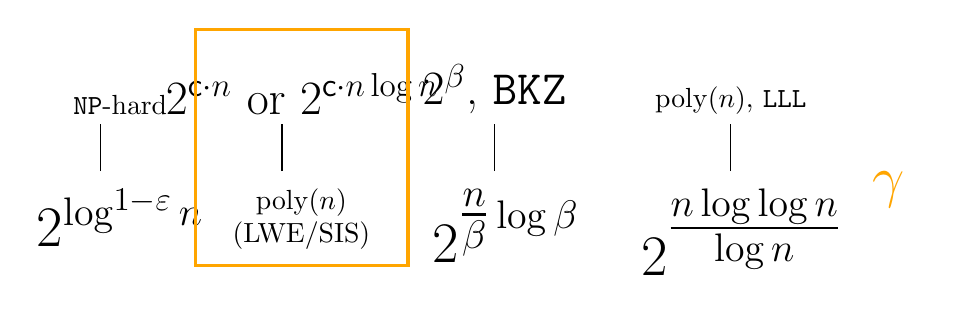
\begin{tikzpicture}
	\centering
	\draw[-stealth, white, thick] (0,0) -- (10.5, 0) node[font=\Large, below, yshift=-5pt]{\huge \color{Orange} $\mathbf{\gamma}$} node[above, yshift=4pt]{Time};
	
	\draw[-] (0.5,-0.3) -- (0.5,0.3) node[above, xshift=7pt] {\texttt{NP}-hard} node[below, yshift=-20pt, align=left, xshift=7pt] {\huge $2^{\log^{1-\eps} n}$};
	
	\draw[-] (2.8,-0.3) -- (2.8,0.3) node[above, xshift=10pt, align=center] {\LARGE $2^{\const  \cdot n}$ or \LARGE $2^{\const  \cdot n \log n}$ } node[below, yshift=-20pt, align=center, xshift=7pt] {$\poly(n)$ \\ (LWE/SIS)};
	
	\draw[-] (5.5,-0.3) -- (5.5,0.3) node[above] {\LARGE $ 2^{\beta}$, \texttt{BKZ}} node[below, yshift=-20pt, align=left, xshift=4pt] {\huge $2^{ \tfrac{n}{\beta} \log \beta} $};
	
	\draw[-] (8.5,-0.3) -- (8.5,0.3) node[above] {$\poly(n)$, \texttt{LLL}} node[below, yshift=-20pt, align=left, xshift=4pt] {\huge $2^{\tfrac{n\log \log n}{\log n}}$};
	
	\pause
	\onslide<2->{
	\draw[draw=Orange, very thick] (1.7, -1.5) rectangle (4.4, 1.5);
	}
	\end{tikzpicture}
	
\end{frame}

\begin{frame}{Practical Algorithms for SVP}

	%2 main families of algorithms for SVP
	
	\begin{itemize}
		\setlength\itemsep{5pt}
		\item {\LARGE{Enumeration}} 
		\onslide<2->{
			\Huge
			\begin{align*}
			\text{Time} = 2^{ ( (1/2e)+\smallo(1) )n \log n}
			\quad \quad \text{Memory} = \poly(n)	
			\end{align*}
			
			\begin{itemize}%[label={$\checkmark$}]
				\large
				\item Lots of improvements for the $\smallo(n \log n)$-term %(Pruning, Random Sampling)
				\item (Somewhat) easy to parallelize
			\end{itemize}
		}
		
		\item {\LARGE{Sieving} (Provable/Heuristic)}
		\onslide<3->{
			\Huge
			\begin{align*}
			&\text{Time} = 2^{(2.465+\smallo(1))n}
			\quad \quad \text{Memory} = 2^{(1.325+\smallo(1))n} \\
			&\text{Time} = 2^{ (0.292+\smallo(1))n}
			\quad \quad \text{Memory} = 2^{ (0.2075+\smallo(1))n}
			\end{align*}
			
			\begin{itemize}%[label={$\checkmark$}]
				\large
				\item Big $\smallo(n)$-factors
				\item Parallelization is painful
				\item Time-memory trade-offs exist
			\end{itemize}
		}
	\end{itemize}

	
\end{frame}

\begin{frame}
Part II \\ [10pt]
\centering
\begin{LARGE}
	
	
	\color{Orange}
	\Huge Kannan-Finke-Pohst Enumeration algorithm
	
\end{LARGE}
\end{frame}


\begin{frame}{Enumeration algorithm for SVP: main idea}
\Large
{\color{Orange} Idea:} enumerate all lattice vector within a ball of certain radius $k$.

\begin{enumerate}
	\item INPUT: basis $B = QR$, $R \in \R^{n \times n}$ -- R-factor \pause
	\item Set $k = \| \bvec_1 \|$ -- a bound 
	\item Let $\xvec \in \Z^n$ be the coefficient vector of $\bvec = B\xvec$. Then
\end{enumerate}
\begin{align*}\label{eq:enum_norm}
\| B\xvec \|^2   = \| R\xvec \|^2 = \| \left( \sum_{i=1}^n r_{1,i}x_i, \sum_{i=2}^n r_{2,i}x_i, \ldots, r_{n,n} x_n \right) \|^2 
 = \sum_{j=1}^n \left( \sum_{i \geq j} r_{j,i} x_i \right)^2.
\end{align*}
\pause
We are going to enumerate $x_i$'s for $i = n, \ldots, 1$, keeping the value $\sum_{j=1}^n \left( \sum_{i \geq j} r_{j,i} x_i \right)^2$ bounded.

\end{frame}

\begin{frame}{Enumeration algorithm for SVP}
\begin{columns}[t]
	\begin{column}{0.3\textwidth}
		\vspace{10pt}
		\begin{tikzpicture}[
		state/.style={circle, fill=white, inner sep=1.8pt},
		]
		%\centering
		\onslide<1>{
			\node [circle, fill=Orange, inner sep=1.8pt] (x11) at (0,0) {};
			\node [circle, fill=Orange, inner sep=1.8pt] (x12) at (1.5,0) {};
			\node [circle, fill=Orange, inner sep=1.8pt] (x13) at (3,0) {};
			\node at (-1.3, 0) {$x_n$};
		}

		\onslide<2>{
			\node [state] (x11) at (0,0) {};
			\node [state] (x12) at (1.5,0) {};
			\node [state] (x13) at (3,0) {};
			\node at (-1.3, 0) {$x_n$};
			
			\node [circle, fill=Orange, inner sep=1.8pt] (x21) at (-0.5,-1.0) {};
			\node [circle, fill=Orange, inner sep=1.8pt] (x22) at (0.9,-1.0) {};
			\node [circle, fill=Orange, inner sep=1.8pt] (x23) at (2.1,-1.0) {};
			\node [circle, fill=Orange, inner sep=1.8pt] (x24) at (3.5,-1.0) {};
			\node at (-1.3, -1.0) {$x_{n-1}$};
			\draw[] (x11) -- (x21);
			\draw[] (x12) -- (x22);
			\draw[] (x12) -- (x23);
			\draw[] (x13) -- (x24);
		}
		\onslide<3>{
			\node [state] (x11) at (0,0) {};
			\node [state] (x12) at (1.5,0) {};
			\node [state] (x13) at (3,0) {};
			\node at (-1.3, 0) {$x_n$};
			
			\node [state] (x21) at (-0.5,-1.0) {};
			\node [state] (x22) at (0.9,-1.0) {};
			\node [state] (x23) at (2.1,-1.0) {};
			\node [state] (x24) at (3.5,-1.0) {};
			\node at (-1.3, -1.0) {$x_{n-1}$};
			\draw[] (x11) -- (x21);
			\draw[] (x12) -- (x22);
			\draw[] (x12) -- (x23);
			\draw[] (x13) -- (x24);
			
			\node [circle, fill=Orange, inner sep=1.8pt] (x31) at (-0.8,-2.5) {};
			\node [circle, fill=Orange, inner sep=1.8pt] (x32) at (-0.2,-2.5) {};
			\node [circle, fill=Orange, inner sep=1.8pt] (x33) at (0.6,-2.5) {};
			\node [circle, fill=Orange, inner sep=1.8pt] (x34) at (1.2,-2.5) {};
			\node [circle, fill=Orange, inner sep=1.8pt] (x35) at (1.8,-2.5) {};
			\node [circle, fill=Orange, inner sep=1.8pt] (x36) at (2.4,-2.5) {};
			\node [circle, fill=Orange, inner sep=1.8pt] (x37) at (3.5,-2.5) {};	
			\node at (-1.3, -2.5) {$x_{n-2}$};
			
			\draw[] (x21) -- (x31);
			\draw[] (x21) -- (x32);
			\draw[] (x22) -- (x33);
			\draw[] (x22) -- (x34);
			\draw[] (x23) -- (x35);
			\draw[] (x23) -- (x36);
			\draw[] (x24) -- (x37);
			
		}
		\onslide<4>
			\node [state] (x11) at (0,0) {};
			\node [state] (x12) at (1.5,0) {};
			\node [state] (x13) at (3,0) {};
			\node at (-1.3, 0) {$x_n$};
			
			\node [state] (x21) at (-0.5,-1.0) {};
			\node [state] (x22) at (0.9,-1.0) {};
			\node [state] (x23) at (2.1,-1.0) {};
			\node [state] (x24) at (3.5,-1.0) {};
			\node at (-1.3, -1.0) {$x_{n-1}$};
			\draw[] (x11) -- (x21);
			\draw[] (x12) -- (x22);
			\draw[] (x12) -- (x23);
			\draw[] (x13) -- (x24);
			
			\node [state] (x31) at (-0.8,-2.5) {};
			\node [state] (x32) at (-0.2,-2.5) {};
			\node [state] (x33) at (0.6,-2.5) {};
			\node [state] (x34) at (1.2,-2.5) {};
			\node [state] (x35) at (1.8,-2.5) {};
			\node [state] (x36) at (2.4,-2.5) {};
			\node [state] (x37) at (3.5,-2.5) {};	
			\node at (-1.3, -2.5) {$x_{n-2}$};
			
			\draw[] (x21) -- (x31);
			\draw[] (x21) -- (x32);
			\draw[] (x22) -- (x33);
			\draw[] (x22) -- (x34);
			\draw[] (x23) -- (x35);
			\draw[] (x23) -- (x36);
			\draw[] (x24) -- (x37);
			\node at (0, -3.0) {$\vdots$};
			\node at (1.5, -3.0) {$\vdots$};
			\node at (3.0, -3.0) {$\vdots$};
			
			\node [state] (x41) at (-1.0,-4.5) {};
			\node [state] (x41) at (-0.6,-4.5) {};			
			\node [state] (x41) at (-0.2,-4.5) {};
			\node [state] (x41) at (0.2,-4.5) {};			
			\node [state] (x41) at (0.6,-4.5) {};	
			\node [state] (x41) at (1.0,-4.5) {};		
			\node [state] (x41) at (1.4,-4.5) {};
			\node [state] (x41) at (1.8,-4.5) {};
			\node [state] (x41) at (2.2,-4.5) {};
			\node [state] (x41) at (2.6,-4.5) {};
			\node [state] (x41) at (3.0,-4.5) {};
			\node [state] (x41) at (3.4,-4.5) {};
			\node [state] (x41) at (3.8,-4.5) {};
			\node at (-1.3, -4.5) {$x_1$};
		%	
		%	\draw[thick, double] (a) -- (b1);
		%	\draw[thick, double] (b1) -- (b2);
		%	\draw[thick, double] (b2) -- (b3);
		\end{tikzpicture}%
	\end{column}%
	\begin{column}{0.1\textwidth}
	\end{column}
	\begin{column}{0.65\textwidth}
		\Large
		\vspace{-5pt} 
		\begin{enumerate}[<+->]
		\itemsep 8pt
		\item Take all 
		$x_n$  $\in \Z$ s.t.\ $| x_n| < \frac{k} {r_{n,n}}$. 
		\item Fix $x_n$. Take all $x_{n-1} \in \Z$ s.t.\ \\  $\left|{x_{n-1} + \frac{r_{n-1,n}}{r_{n-1,n-1}}x_n }\right| < \left( \frac{k^2-(r_{n,n}x_n )^2}{r_{n-1, n-1}}\right)^{1/2}$ 
		\item For fixed $x_n, x_{n-1}$, take all `legitimate' $x_{n-2} \in \Z$ 
		\item Continue all the way to $x_1$'s.
	\end{enumerate}
	\end{column}
	
\end{columns}

\end{frame}

\begin{frame}{Complexity}
	\Large
	\begin{theorem} The size of the enumeration tree of the above algorithm that receives on input an LLL-reduced basis $B$ of an $n$-dimensional lattice	is $2^{\O(n^2)}$. It can be traversed using $\poly(n)$ memory.
	\end{theorem}

A proof to be shown in TD.

\vspace{15pt}

One can tweak the algorithm by making the smallest $r_{i,i}$'s larger. This gives the enumeration tree to the size $2^{\frac{n \log n}{2e}+o(n)}$, {\color{Orange}[Kan83,HanSte07] }


\end{frame}


\begin{frame}
	\renewcommand\footnoterule{}
	Part III \\ [10pt]
	\begin{center}
		\color{Orange} \Huge{Sieving}
		
		\vspace{20pt}
		
		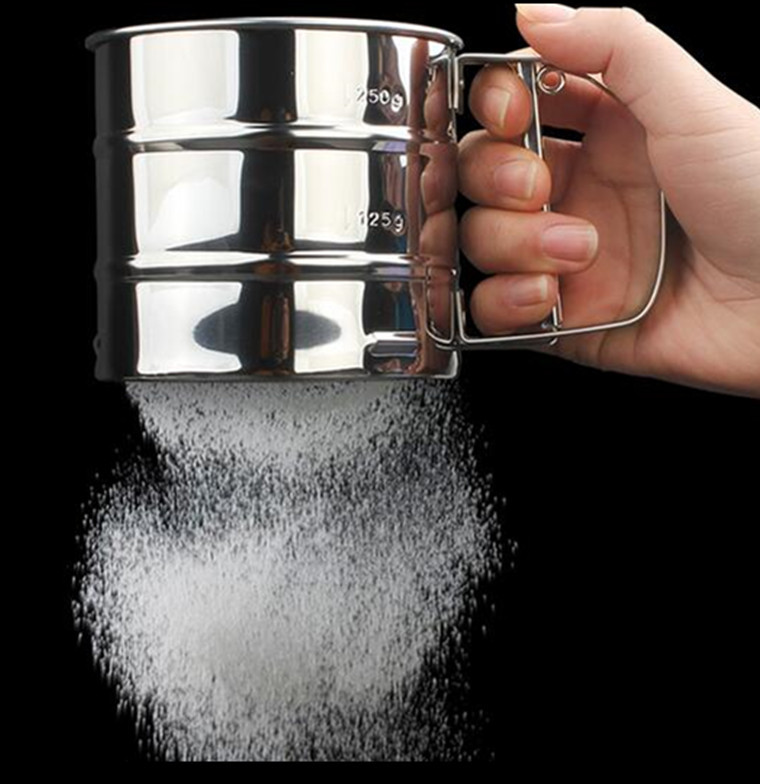
\includegraphics[width=4.0cm]{siever.jpg}
		\blfootnote{{\color{gray}https://sites.google.com/a/x.bestledlights.cf/a223/1-32772214555}}
	\end{center}
	
\end{frame}

%\section{Sieving algorithms}

\begin{frame}{Basic 2-Sieve (Nguyen-Vidick sieve)}
\vspace{-5pt}
\Large
{\color{Orange}Main idea} in all sieving algorithms: {\color{Orange}saturate} space with enough lattice vectors so that their sums give short(er) vectors
\centering
	\begin{tabular}{@{}c @{}c }
		\hspace{-30pt}
		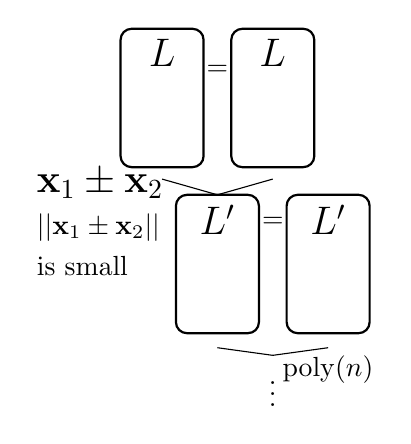
\begin{tikzpicture}
		%\vspace*{-50pt}
		\centering
		\onslide<1->{
			\draw[rounded corners, thick] (0pt, 0pt) rectangle (30pt, 50pt) node(L1)[xshift=-15pt, below]{\Large $L$};
			\draw[rounded corners, thick] (40pt, 0pt) rectangle (70pt, 50pt)node(L2)[xshift=-15pt, below]{\Large $L$};
			\node[draw=none] at (35pt, 35pt){$=$};
		}
		\pause
		\onslide<3->{
			\draw[rounded corners, thick] (20pt, -60pt) rectangle (50pt, -10pt) node(L3)[xshift=-15pt, below]{\Large $L'$};
			
			\draw[-] ([yshift=-37pt]L1.south) -- (L3.north) node[left, xshift=-16pt,yshift=-10pt, align=left]{\Large $\xvec_1 \pm \xvec_2$ \\[3pt] $||\xvec_1 \pm \xvec_2||$\\[3pt] is small};
			\draw[-] ([yshift=-37pt]L2.south) -- (L3.north);
		}
		\pause
		
		\onslide<4->{
			\draw[rounded corners, thick] (60pt, -60pt) rectangle (90pt, -10pt) node(L4)[xshift=-15pt, below]{\Large $L'$};
			\node[draw=none] at (55pt, -20pt){$=$};
		}
			\pause
		\onslide<5->
		{
			\draw[-] ([yshift=-37pt]L3.south) -- (55pt, -68pt) node[below]{$\vdots$} node[right, yshift=-5pt]{$\poly(n)$};
			\draw[-] ([yshift=-37pt]L4.south) -- (55pt, -68pt);
		}
		
		%\onslide<4>{
		%	\node[below, text width=3.5cm, xshift=5cm] at (85pt,10pt) {Memory: $2^{\bigO(n)}$};
		%}
		
		%\pause
		%\node[below, text width=3.5cm, xshift=5cm, font=\bfseries, color=red] at (85pt,10pt) {Memory: $2^{\bigO(n)}$};
		\end{tikzpicture} &
		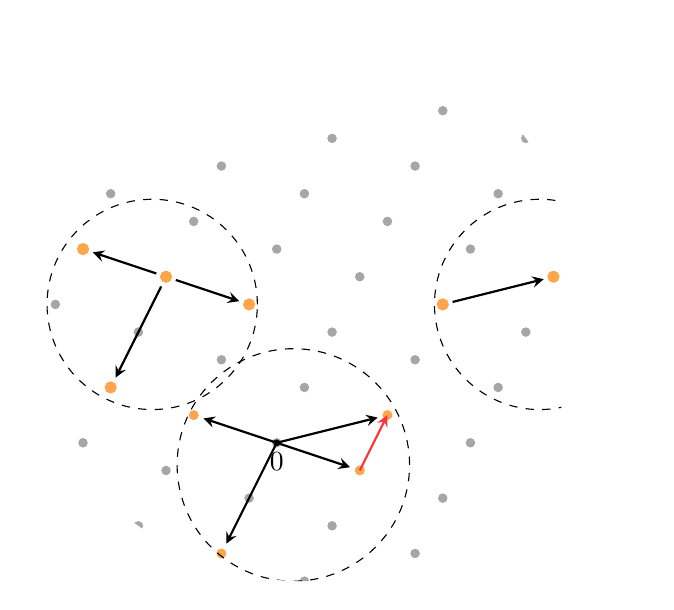
\begin{tikzpicture}
		%\begin{scope}
		\onslide<1->{
			\clip (10pt,50pt) circle (100pt);
			\foreach \y in {-3,...,6}
			\foreach \x in {-5,...,5}
			\filldraw[gray!70](\x*40pt+\y*10pt, 10pt*\x+20pt*\y) circle (1.5pt);
			
			\filldraw(0pt,0pt) circle (1pt) node[below] (zero) { $0$};
		}
		
		\onslide<1-2>{
			\filldraw[orange!70](-40pt, 60pt) circle(2.0pt) node (v1) {};
			\filldraw[orange!70](-10pt, 50pt) circle(2.0pt) node (v2) {};
			\filldraw[orange!70](-70pt, 70pt) circle(2.0pt) node (v3) {};
			\filldraw[orange!70](-60pt, 20pt) circle(2.0pt) node (v4) {};
			
			\filldraw[orange!70](60pt, 50pt) circle(2.0pt) node (v5) {};
			\filldraw[orange!70](100pt, 60pt) circle(2.0pt) node (v6) {};
			
			%\filldraw(50pt, 100pt) circle(1.3pt) node (v7) {};
			%\filldraw(40pt, 80pt) circle(1.3pt) node (v8) {};
		}
		
		\onslide<2>{
			\draw[-stealth, thick] (v1) -- (v2);
			\draw[-stealth, thick] (v1) -- (v3);
			\draw[-stealth, thick] (v1) -- (v4);
			
			\draw[dashed] ([shift=({-5pt,-10pt})]v1) circle (38pt);
			
			\draw[-stealth, thick] (v5) -- (v6);
			\draw[dashed] ([shift=({-5pt,-10pt})]v6) circle (38pt);
			
			%\draw[->, thick] (v8) -- (v7);
			%\draw[dashed] ([shift=({-20pt,5pt})]v7) circle (38pt);
		}
		
		\onslide<3->{
			\filldraw[orange!70](30pt, -10pt) circle(1.5pt) node (v1v2){};
			\filldraw[orange!70](-30pt, 10pt) circle(1.5pt) node (v1v3){};
			\filldraw[orange!70](-20pt, -40pt) circle(1.5pt) node (v1v4){};
			
			\filldraw[orange!70](40pt, 10pt) circle(1.5pt) node (v5v6){};
			
			%\filldraw[orange!70](10pt, 20pt) circle(1.5pt) node (v7v8){};
			
			\draw[-stealth, thick] (zero.north) -- (v1v2);
			\draw[-stealth, thick] (zero.north) -- (v1v3);
			\draw[-stealth, thick] (zero.north) -- (v1v4);
			
			\draw[-stealth, thick] (zero.north) -- (v5v6);
		}
		
		\onslide<3>{
			\filldraw[orange!70](30pt, -10pt) circle(1.5pt) node (v1v2){};
			\filldraw[orange!70](-30pt, 10pt) circle(1.5pt) node (v1v3){};
			\filldraw[orange!70](-20pt, -40pt) circle(1.5pt) node (v1v4){};
			
			\filldraw[orange!70](40pt, 10pt) circle(1.5pt) node (v5v6){};
			
			%\filldraw[orange!70](10pt, 20pt) circle(1.5pt) node (v7v8){};	
			
			\draw[dashed] ([shift=({6pt,-8pt})]zero.north)  circle (42pt);
		}
		\onslide<5->{
			%\filldraw[red!80]  circle(1.5pt)  {};
			\draw[-stealth, thick, red!80] (30pt, -10pt) -- (40pt, 10pt);
		}
		
%		\onslide<6->
%		{
%			\draw[draw=CharCoalDark,fill=CharCoalDark] (-2.6,1.0) rectangle (4,3.0) node[pos=0.5, color=white,align=left]{
%							 \Huge $|L| = \softO(  2^{0.2075n} )$ \\ [7pt]
%							 \Huge $T(\text{\Large naive 2-Sieve}) =\softO( |L|^2)$
%			};
%		}
		%\end{scope}
		\end{tikzpicture}
	\end{tabular}
\end{frame}

\begin{frame}{How large $|L|$ should be?}
	\pause
	Assumption: vectors (normalized) in $|L|$ are uniform iid on $S^{n-1}$. \\
	
	\tikzmark{start}
	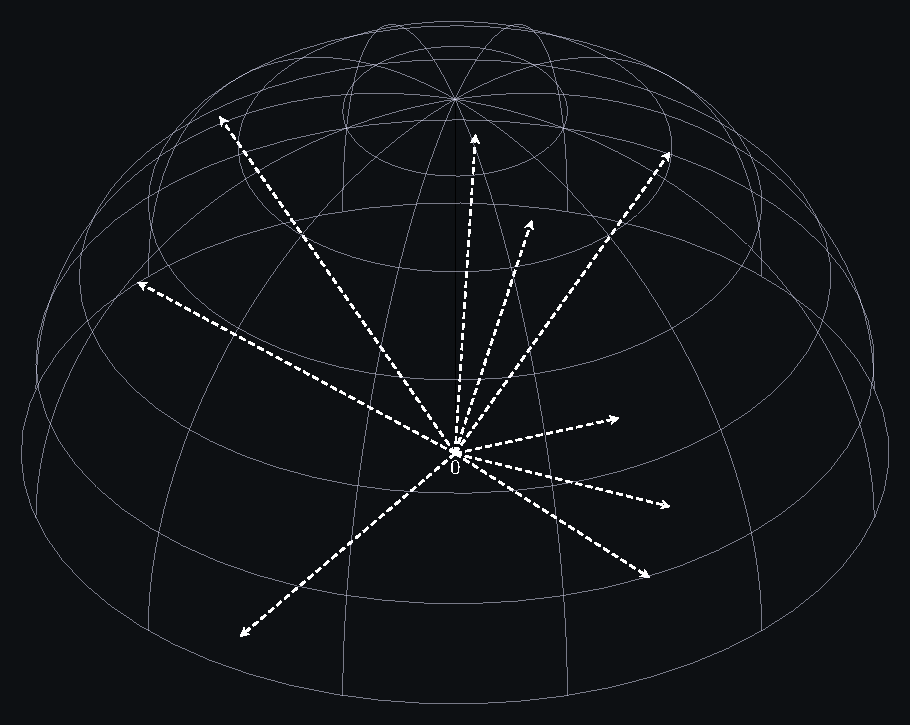
\includegraphics[width=\textwidth]{semi-sphere1}
	\tikzmark{end}
\end{frame}
\begin{frame}{How large $|L|$ should be?}
Assumption: vectors (normalized) in $|L|$ are uniform iid on $S^{n-1}$. \\

\tikzmark{start}
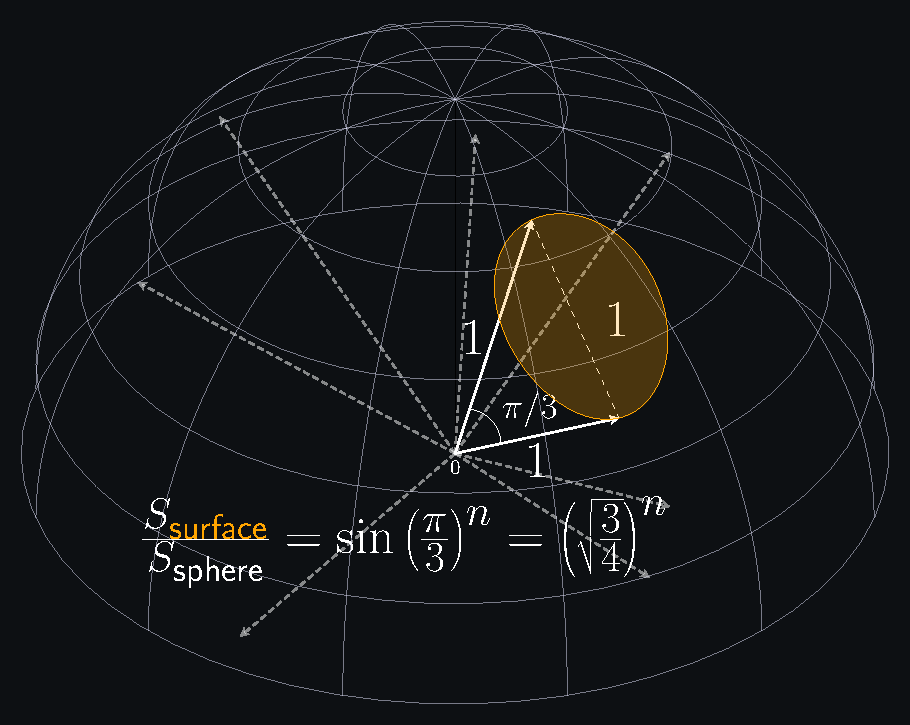
\includegraphics[width=\textwidth]{semi-sphere2}
\tikzmark{end}
\end{frame}

\begin{frame}{Basic 2-Sieve (Nguyen-Vidick sieve)}
\Large
{\color{Orange}Main idea} in all sieving algorithms: {\color{Orange}saturate} space with enough lattice vectors so that their sums give short(er) vectors
\centering
\begin{tabular}{@{}c @{}c }
	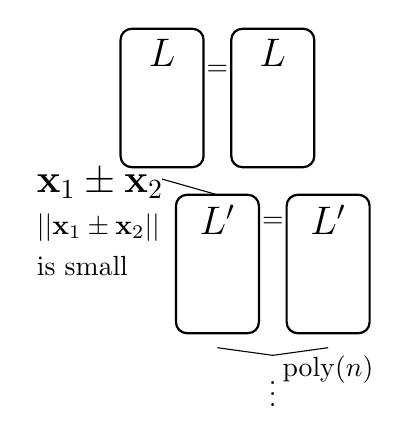
\begin{tikzpicture}
	\vspace*{-40pt}
	\centering
		\draw[rounded corners, thick] (0pt, 0pt) rectangle (30pt, 50pt) node(L1)[xshift=-15pt, below]{\Large $L$};
		\draw[rounded corners, thick] (40pt, 0pt) rectangle (70pt, 50pt)node(L2)[xshift=-15pt, below]{\Large $L$};
		\node[draw=none] at (35pt, 35pt){$=$};

		\draw[rounded corners, thick] (20pt, -60pt) rectangle (50pt, -10pt) node(L3)[xshift=-15pt, below]{\Large $L'$};
		
		\draw[-] ([yshift=-37pt]L1.south) -- (L3.north) node[left, xshift=-16pt,yshift=-10pt, align=left]{\Large $\xvec_1 \pm \xvec_2$ \\[3pt] $||\xvec_1 \pm \xvec_2||$\\[3pt] is small};
	
		\draw[rounded corners, thick] (60pt, -60pt) rectangle (90pt, -10pt) node(L4)[xshift=-15pt, below]{\Large $L'$};
		\node[draw=none] at (55pt, -20pt){$=$};
	
		\draw[-] ([yshift=-37pt]L3.south) -- (55pt, -68pt) node[below]{$\vdots$} node[right, yshift=-5pt]{$\poly(n)$};
		\draw[-] ([yshift=-37pt]L4.south) -- (55pt, -68pt);
	\end{tikzpicture} &
	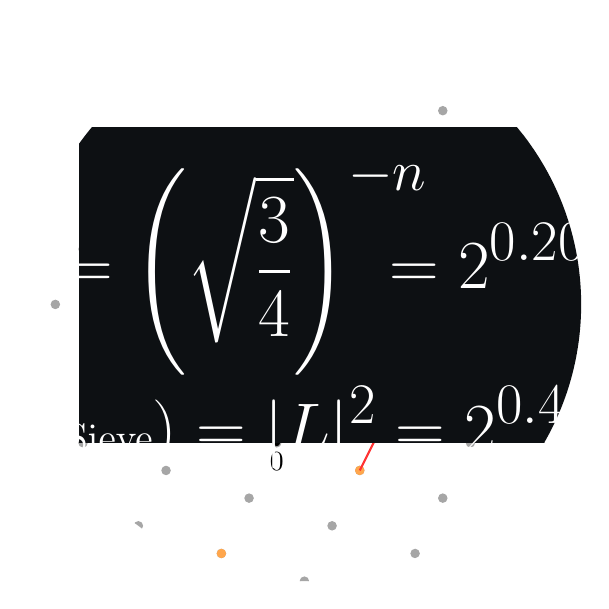
\begin{tikzpicture}
		\clip (10pt,50pt) circle (100pt);
		\foreach \y in {-3,...,6}
		\foreach \x in {-5,...,5}
		\filldraw[gray!70](\x*40pt+\y*10pt, 10pt*\x+20pt*\y) circle (1.5pt);
		
		\filldraw(0pt,0pt) circle (1pt) node[below] (zero) { $0$};


		\filldraw[orange!70](30pt, -10pt) circle(1.5pt) node (v1v2){};
		\filldraw[orange!70](-30pt, 10pt) circle(1.5pt) node (v1v3){};
		\filldraw[orange!70](-20pt, -40pt) circle(1.5pt) node (v1v4){};
		
		\filldraw[orange!70](40pt, 10pt) circle(1.5pt) node (v5v6){};
		
		\filldraw[orange!70](10pt, 20pt) circle(1.5pt) node (v7v8){};	
		

		\draw[-stealth, thick, red!80] (30pt, -10pt) -- (40pt, 10pt);

		\draw[draw=CharCoalDark,fill=CharCoalDark] (-2.5,-0.0) rectangle (5,4.0) node[pos=0.4, color=white]{
			\Huge
			$
			\begin{aligned}
			&\Huge |L| = \left(\sqrt{\frac{3}{4}}\right)^{-n} \mkern-15mu = 2^{0.2075n} \\
			&\Huge T(\text{\Large 2-Sieve})  =|L|^2  = 2^{0.415n} 
			\end{aligned}
			$
	};
	%\end{scope}
	\end{tikzpicture}
\end{tabular}
\end{frame}

\begin{frame}{SVP: conclusions}
	\Large
	\begin{itemize}
		\itemsep 8pt
		\item Best known SVP algorithm require at least exponential (in lattice dimension) time
		\item We do not know how to use the additional structure to significantly speed up SVP algorithms for algebraic lattices
	\end{itemize}
	\vspace{10pt}
	
	\centering {\color{Orange} Open questions}
	\begin{itemize}
		\item SVP in $\ell_\infty$ norm, algebraic SVP
		\item Precise complexity of SVP taking into account memory costs
		\item Quantum speed ups for SVP/LWE/SIS?
	\end{itemize}
\end{frame}

\begin{frame}
Part IV \\ [10pt]
\centering
\begin{LARGE}
	
	
	\color{Orange}
	\Huge Block Korkine-Zolotarev (BKZ) algorithm
	
\end{LARGE}
\vspace{40pt}
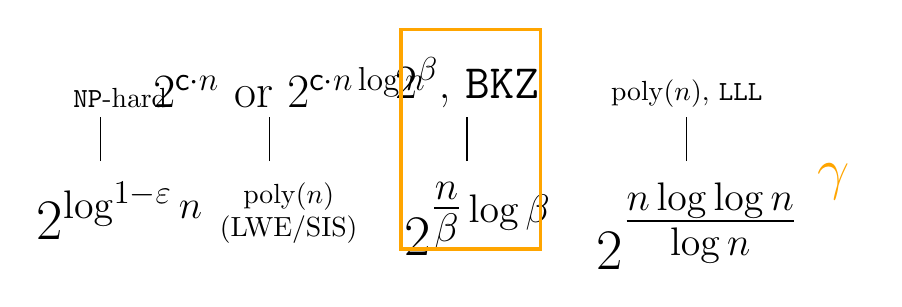
\begin{tikzpicture}[scale=0.93]

\draw[-stealth, white, thick] (0,0) -- (10.5, 0) node[font=\Large, below, yshift=-5pt]{\huge \color{Orange} $\mathbf{\gamma}$} node[above, yshift=4pt]{Time};

\draw[-] (0.5,-0.3) -- (0.5,0.3) node[above, xshift=7pt] {\texttt{NP}-hard} node[below, yshift=-20pt, align=left, xshift=7pt] {\huge $2^{\log^{1-\eps} n}$};

\draw[-] (2.8,-0.3) -- (2.8,0.3) node[above, xshift=10pt, align=center] {\LARGE $2^{\const  \cdot n}$ or \LARGE $2^{\const  \cdot n \log n}$ } node[below, yshift=-20pt, align=center, xshift=7pt] {$\poly(n)$ \\ (LWE/SIS)};

\draw[-] (5.5,-0.3) -- (5.5,0.3) node[above] {\LARGE $ 2^{\beta}$, \texttt{BKZ}} node[below, yshift=-20pt, align=left, xshift=4pt] {\huge $2^{ \tfrac{n}{\beta} \log \beta} $};

\draw[-] (8.5,-0.3) -- (8.5,0.3) node[above] {$\poly(n)$, \texttt{LLL}} node[below, yshift=-20pt, align=left, xshift=4pt] {\huge $2^{\tfrac{n\log \log n}{\log n}}$};


\draw[draw=Orange, very thick] (4.6, -1.5) rectangle (6.5, 1.5);
\end{tikzpicture}

\end{frame}

\begin{frame}{Small improvement at a time}
\LARGE
\begin{itemize}
	\setlength\itemsep{5pt}
	
	\item We never call an SVP oracle on an non-preprocessed basis
	\item Having a ``better quality'' basis of $\mathcal{L}$ is beneficial for most (all?) algorithms
	\item We try to gradually improve the ``quality'' of a basis
\end{itemize}
{\color{Orange} Quality} - length of Gram-Schmidt vectors
\end{frame}

\begin{frame}{Projected lattice}
\centering
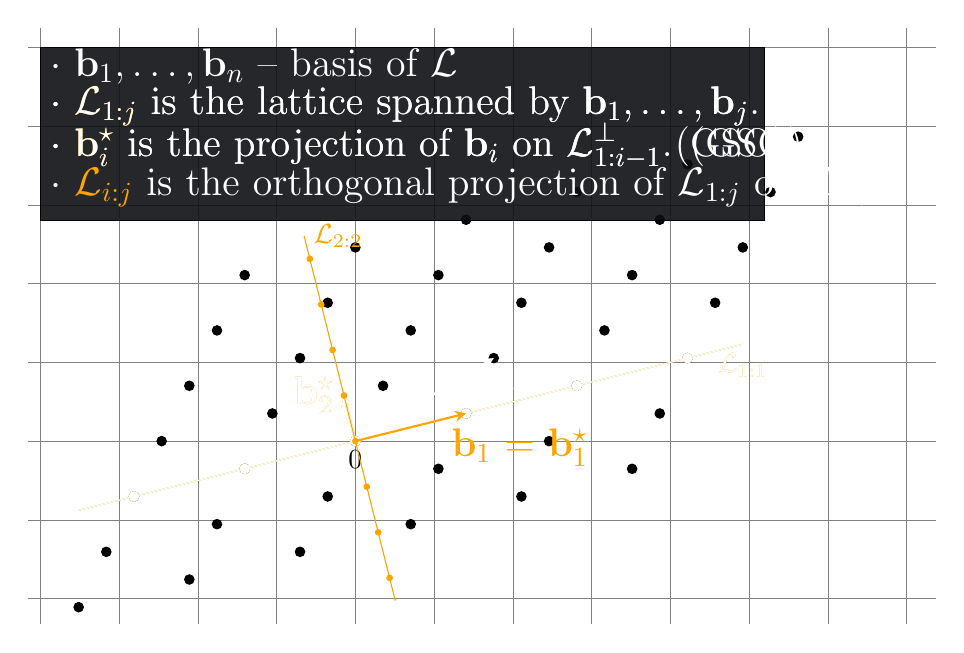
\begin{tikzpicture}[show background grid]
\begin{scope}
\foreach \y in {-2,...,4}
\foreach \x in {-2,...,3}
\filldraw(\x*40pt+\y*10pt, 10pt*\x+20pt*\y) circle (1.7pt);
\filldraw(0pt,0pt) node[below]{ $0$};

\draw[-stealth, white, thick] (0,0) -- (50pt, 30pt) node[font=\Large, below, xshift=5pt]{$\bvec_2$};
\draw[-stealth, white, thick] (0,0) -- (40pt, 10pt) node[font=\Large, below, xshift=2pt, yshift = -2pt]{$\bvec_1$};

\onslide<2>{
\foreach \x in {-2,...,3}
\filldraw[color = Orange](\x*40pt, \x*10pt) circle (1.7pt);
\draw[Orange, thin] (-100pt,-25pt) -- (140pt,35pt) node[below] {$\L_{1:1}$};
}

\onslide<3->{
\foreach \x in {-2,...,3}
\filldraw[color = white](\x*40pt, \x*10pt) circle (1.7pt);
\draw[color=white, thin] (-100pt,-25pt) -- (140pt,35pt) node[below] {$\L_{1:1}$};
}

\onslide<3>{
\draw[-stealth, Orange, thick] (0,0) -- (40pt, 10pt) node[font=\Large, below, xshift=2pt, yshift = -2pt]{$\bvec_1$\rlap{\smash{ = \color{Orange} $\bvec_1^\star$}}};
}


\onslide<3>{
\draw[-stealth, Orange, thick] (0,0) -> (-4.1176pt, 16.47pt) node[font = \Large, left]{$ \bvec_2^\star$};  %7/17 * (-10,40)
}
\onslide<4->{
\draw[-stealth, white, thick] (0,0) -> (-4.1176pt, 16.47pt) node[font = \Large, left]{$ \bvec_2^\star$};  %7/17 * (-10,40)
}

\onslide<4>{
\foreach \x in {-3,...,4}
\filldraw[color = Orange](\x * -4.1176pt, \x * 16.47pt) circle (1pt);
\draw[Orange, thin] (-3.5 *-4.1176pt, -3.5 * 16.47pt) -- (4.5 *-4.1176pt, 4.5 * 16.47pt) node[right] {$\L_{2:2}$};
}

\draw[fill=CharCoalDark, opacity=0.9] (-4,5) rectangle (5.2,2.8);
\node[font = \Large, right, yshift = -7pt, color=white, opacity=1] at (-4,5) {$\cdot$ $\bvec_1,\ldots, \bvec_n$ -- basis of $\L$};
\onslide<2>{\node[font = \Large, right, yshift = -7pt, color=white, opacity=1] at (-4,4.5) {$\cdot$ {\color{Orange}$\L_{1:j}$} is the lattice spanned by $\bvec_1,\ldots,\bvec_j$};}
\onslide<3->{\node[font = \Large, right, yshift = -7pt, color=white, opacity=1] at (-4,4.5) {$\cdot$ {$\L_{1:j}$} is the lattice spanned by $\bvec_1,\ldots,\bvec_j$.};}
\onslide<3>{\node[font = \Large, right, yshift = -7pt, color=white, opacity=1] at (-4,4) {$\cdot$ {\color{Orange}$ \bvec_i^\star$} is the projection of $\bvec_i$ on $\L_{1:{i-1}}^{\perp}$. (GSO)};}
\onslide<4->{\node[font = \Large, right, yshift = -7pt, color=white, opacity=1] at (-4,4) {$\cdot$ $\bvec_i^\star$ is the projection of $\bvec_i$ on $\L_{1:{i-1}}^{\perp}$ (GSO)};}
\onslide<4>{\node[font = \Large, right, yshift = -7pt, color=white, opacity=1] at (-4,3.5) {$\cdot$ {\color{Orange}$\L_{i:j}$} is the orthogonal projection of $\L_{1:j}$ on $\L_{1:i-1}^{\perp}$.};}
% 	\onslide<5->{\node[font = \Large, right, yshift = -7pt, color=white, opacity=1] at (-4,3.5) {Let $\L_{i:j}$ be the orthogonal projection of $\L_{1:j}$ on $\L_{1:i-1}^{\perp}$.};}
%};}
\end{scope}
%\draw[CharCoalDark] (-5,-4) rectangle (6,-1.9) node[pos=.5, color=white, opacity=1,align=left] {\Large A lattice $\mathcal{L}$ -- a set of all integer linear combination of basis vectors $\{ \vec{b}_1, \ldots, \vec{b}_n\}$ \\
%Usually, $\vec{b}_i \in \Z^n.$};
\end{tikzpicture}
\end{frame}


\renewcommand{\tikzmark}[1]{\tikz[overlay,remember picture,baseline=(#1.base)]
\node (#1) {\strut};}
\begin{frame}[fragile]{BKZ (simplified)}
\LARGE Notation: $\mathcal{L}_{[\ell \; ; \; r]}$ - orthogonal projection of $\mathcal{L}_{1:r}$ on $\mathcal{L}^\perp_{1:\ell-1}$
\vspace{20pt}

\begin{columns}[T] % align columns
\begin{column}{.55\textwidth}
\Large
\only<1>{
	\textbf{ Input:} $B = (\bvec_i), \beta$
	\begin{algorithmic}
		\For{$k = 2 \ldots n-1$}
		\State {\color{Orange} $\bvec$} $\gets $ \Call{SVP}{$\mathcal{L}_{[k\; ;\; \min\{k+\beta-1, n\}]}$}
		\EndFor
		\If{{\color{Orange} $\bvec$} is ``short enough''}
		\State Insert {\color{Orange} $\bvec$} into $B$
		\State Remove lin.\ dependencies
		\EndIf
	\end{algorithmic}
}
\only<2>{
	\textbf{ Input:} $B = (\bvec_i), \beta$
	\begin{algorithmic}
		\For{{\color{Orange} $k =2$}}
		\State {\color{Orange} $\bvec$} $\gets $ \Call{SVP}{$\mathcal{L}_{[2\; ;\; \min\{\beta+1, n\}]}$}
		\EndFor
		\If{{\color{Orange} $\bvec$} is ``short enough''}
		\State Insert {\color{Orange} $\bvec$} into $B$
		\State Remove lin.\ dependencies
		\EndIf
	\end{algorithmic}
}

\only<3>{
	\textbf{ Input:} $B = (\bvec_i), \beta$
	\begin{algorithmic}
		\For{{\color{Orange} $k=3$}}
		\State {\color{Orange} $\bvec$} $\gets $ \Call{SVP}{$\mathcal{L}_{[3\; ;\; \min\{\beta+2, n\}]}$}
		\EndFor
		\If{{\color{Orange} $\bvec$} is ``short enough''}
		\State Insert {\color{Orange} $\bvec$} into $B$
		\State Remove lin.\ dependencies
		\EndIf
	\end{algorithmic}
}

\only<4>{
	\textbf{ Input:} $B = (\bvec_i), \beta$
	\begin{algorithmic}
		\For{{\color{Orange} $k=4$}}
		\State {\color{Orange} $\bvec$} $\gets $ \Call{SVP}{$\mathcal{L}_{[4\; ;\; \min\{\beta+3, n\}]}$}
		\EndFor
		\If{{\color{Orange} $\bvec$} is ``short enough''}
		\State Insert {\color{Orange} $\bvec$} into $B$
		\State Remove lin.\ dependencies
		\EndIf
	\end{algorithmic}
}

\only<5>{
	\textbf{ Input:} $B = (\bvec_i), \beta$
	\begin{algorithmic}
		\For{$k = 1 \ldots n-1$}
		\State {\color{Orange} $\bvec$} $\gets $ \Call{SVP}{$\mathcal{L}_{[k\; ;\; \min\{k+\beta-1, n\}]}$}
		\EndFor
		\If{{\color{Orange} $\bvec$} is ``short enough''}
		\State Insert {\color{Orange} $\bvec$} into $B$
		\State Remove lin.\ dependencies
		\EndIf
	\end{algorithmic}
}

%		\only<5>{
%			\textbf{ Input:} $B = (\bvec_i), \beta$
%			\begin{algorithmic}
%				\For{$k = 1 \ldots n-1$}
%				\State {\color{Orange} $\bvec_1, \ldots \bvec_\beta$} $\gets $ \Call{HKZ}{$\mathcal{L}_{[k\; ;\; \min\{k+\beta-1, n\}]}$}
%				\EndFor
%				\If{{\color{Orange} $\bvec_1$} is ``short enough''}
%				\State Insert {\color{Orange} $\bvec_1$} into $B$
%				\State Remove lin.\ dependencies
%				\EndIf
%			\end{algorithmic}
%		}
\end{column}%
\begin{column}{.48\textwidth}
\only<1>{
	\[
	\arraycolsep=1.7pt
	\left (
	\begin{array}{c c c c c c c c}
	\rule{1pt}{10pt} & \rule{1pt}{10pt} &  \rule{1pt}{10pt}  & & \rule{1pt}{10pt} & \rule{1pt}{10pt} &  & \rule{1pt}{10pt} \\
	\bvec_1 & \bvec_2 & \bvec_3 & ... & \bvec_{\beta} & \bvec_{\beta+1} & ... & \bvec_n \\
	\rule{1pt}{10pt} & \rule{1pt}{10pt} &  \rule{1pt}{10pt} & & \rule{1pt}{10pt} & \rule{1pt}{10pt} &  & \rule{1pt}{10pt} \\
	\end{array}
	\right )
	\]
	
	%\begin{tikzpicture}[overlay, remember picture,decoration={brace,amplitude=5pt}]
	%\draw[decorate,thick] (upper1.north) -- (upper2.north)
	%node [midway,above=5pt] {Right block};
	%\end{tikzpicture}
}
\only<2>{
	\[
	\arraycolsep=1.7pt
	\left (
	\begin{array}{c c c c c c c c}
	\rule{1pt}{10pt} & \rule{1pt}{10pt} &  \rule{1pt}{10pt}  & & \rule{1pt}{10pt} & \rule{1pt}{10pt} &  & \rule{1pt}{10pt} \\
	\bvec_1 & \bvec_2 & \bvec_3 & ... & \bvec_{\beta} & \bvec_{\beta+1} & ... & \bvec_n \\
	\rule{1pt}{10pt} & \rule{1pt}{10pt} &  \rule{1pt}{10pt} & & \rule{1pt}{10pt} & \rule{1pt}{10pt} &  & \rule{1pt}{10pt} \\
	\end{array}
	\right )
	\]
	
	\begin{tikzpicture}[overlay, remember picture,decoration={brace,amplitude=8pt, mirror}]
	\draw[decorate,thick] (0.6,0) -- (2.8,0) node [midway,below=10pt] {SVP};
	\end{tikzpicture}
}

\only<3>{
	\[
	\arraycolsep=1.7pt
	\left (
	\begin{array}{c c c c c c c c}
	\rule{1pt}{10pt} & \rule{1pt}{10pt} &  \rule{1pt}{10pt}  & & \rule{1pt}{10pt} & \rule{1pt}{10pt} &  & \rule{1pt}{10pt} \\
	\color{Orange}\bvec_1 & \bvec_2 & \bvec_3 & ... & \bvec_{\beta} & \bvec_{\beta+1} & ... & \bvec_n \\
	\rule{1pt}{10pt} & \rule{1pt}{10pt} &  \rule{1pt}{10pt} & & \rule{1pt}{10pt} & \rule{1pt}{10pt} &  & \rule{1pt}{10pt} \\
	\end{array}
	\right )
	\]
	
	\begin{tikzpicture}[overlay, remember picture,decoration={brace,amplitude=8pt, mirror}]
	\draw[decorate,thick] (1.3,0) -- (3.6,0) node [midway,below=10pt] {SVP};
	\end{tikzpicture}
}

\only<4>{
	\[
	\arraycolsep=1.7pt
	\left (
	\begin{array}{c c c c c c c c}
	\rule{1pt}{10pt} & \rule{1pt}{10pt} &  \rule{1pt}{10pt}  & & \rule{1pt}{10pt} & \rule{1pt}{10pt} &  & \rule{1pt}{10pt} \\
	\bvec_1 & \color{orange}\bvec_2 & \bvec_3 & ... & \bvec_{\beta} & \bvec_{\beta+1} & ... & \bvec_n \\
	\rule{1pt}{10pt} & \rule{1pt}{10pt} &  \rule{1pt}{10pt} & & \rule{1pt}{10pt} & \rule{1pt}{10pt} &  & \rule{1pt}{10pt} \\
	\end{array}
	\right )
	\]
	
	\begin{tikzpicture}[overlay, remember picture,decoration={brace,amplitude=8pt, mirror}]
	\draw[decorate,thick] (1.8,0) -- (4.1,0) node [midway,below=10pt] {SVP};
	\end{tikzpicture}
}

\only<5>{
	\[
	\arraycolsep=1.7pt
	\left (
	\begin{array}{c c c c c c c c}
	\rule{1pt}{10pt} & \rule{1pt}{10pt} &  \rule{1pt}{10pt}  & & \rule{1pt}{10pt} & \rule{1pt}{10pt} &  & \rule{1pt}{10pt} \\
	\bvec_1 & \bvec_2 & \color{orange}\bvec_3 & ... & \bvec_{\beta} & \bvec_{\beta+1} & ... & \bvec_n \\
	\rule{1pt}{10pt} & \rule{1pt}{10pt} &  \rule{1pt}{10pt} & & \rule{1pt}{10pt} & \rule{1pt}{10pt} &  & \rule{1pt}{10pt} \\
	\end{array}
	\right )
	\]
	
	\begin{tikzpicture}[overlay, remember picture,decoration={brace,amplitude=8pt, mirror}]
	\draw[decorate,thick] (2.7,0) -- (4.8,0) node [midway,below=10pt] {SVP};
	\end{tikzpicture}
}
\end{column}%
\end{columns}

\pause
\large 

\begin{itemize}
	\item BKZ runs this FOR-loop while there has been a change in the basis
	\item one run of this FOR-loop is called {\color{Orange} a tour}
\end{itemize}

\end{frame}

\begin{frame}{BKZ: Output Quality and Runtime}
	\LARGE
	\begin{itemize}
		\itemsep  8pt
		\item The running time of the algorithm is dominated by the SVP calls if we bound the number of tours by $\poly(n)$. 
		\item This leads to the complexity $2^{\bigO(\beta)}$ when sieving is used for SVP and $2^{\bigO(\beta\log \beta)}$. Question: memory?
		\item The approximation factor achieved by BKZ is (see TD):
		\[
		\|  \bvec_1   \| \leq \beta^{\frac{n-1}{\beta-1}}\lambda_1(L).
		\]
	\end{itemize}
\end{frame}

\begin{frame}{Time to show the demo...}
\url{TODO}
\end{frame}

\begin{frame}
Part V \\ [10pt]
\begin{center}
	\color{Orange} \Huge{Solving LWE with BKZ}
	
\end{center}
\end{frame}





\begin{frame}{LWE is BDD}
\vspace{-8pt}
\centering
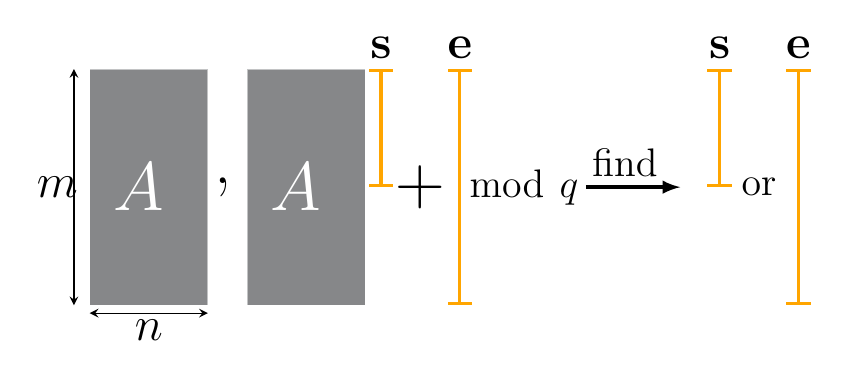
\begin{tikzpicture}
\draw[fill=CharCoalDark, draw=white, opacity=0.5] (-6.0,4.0) rectangle (-4.5,7.0) node[color=white, opacity=1,align=center, pos=0.5] {
	\Huge  $A$
}; 
\draw[stealth-stealth] (-6.2,4.0) -- (-6.2,7.0) node[midway, xshift=-6pt] {\LARGE $m$};
\draw[stealth-stealth] (-6.0,3.9) -- (-4.5,3.9) node[midway, yshift=-6pt] {\LARGE $n$};

\draw(-4.3, 5.5)node{\Huge ,};

\draw[fill=CharCoalDark, draw=white, opacity=0.5] (-4.0,4.0) rectangle (-2.5,7.0) node[color=white, opacity=1,align=center, pos=0.5] {
	\Huge  $A$
}; 

\draw[|-|, draw=Orange, very thick] (-2.3, 5.5) -- (-2.3, 7.0) node[above]{\LARGE $\svec$};

\draw(-1.8, 5.5)node{\Huge $+$};

\draw[|-|, draw=Orange, very thick] (-1.3, 4.0) -- (-1.3, 7.0) node[above]{\LARGE $\evec$};

\draw(-0.5, 5.5)node{\Large $\bmod~q$};
\draw[-latex, very thick] (0.3, 5.5) -- (1.5, 5.5) node[above, xshift=-20pt]{\Large find};

\draw[|-|, draw=Orange, very thick] (2.0, 5.5) -- (2.0, 7.0) node[above]{\LARGE $\svec$};
\draw(2.5, 5.5)node{\Large or};
\draw[|-|, draw=Orange, very thick] (3.0, 4.0) -- (3.0, 7.0) node[above]{\LARGE $\evec$};
\end{tikzpicture}
\Large
\vspace{-10pt}
\begin{itemize}
	\setlength\itemsep{9pt}
	\item $A$ defines the Construction-A lattice
	\[
	\Lat_q(A) = A\Z_q^n + q\Z^m
	\]
	\item W.h.p., $\Lat_q(A)$ is of dim. $m$ and $\det(\Lat_q(A)) = q^{m-n}$.
	\item $As +e \bmod~q$ is a point near $\Lat_q(A)$ at distance $\Theta(\sqrt{m} \alpha q)$
	\item $(A,As+e)$ is a {\color{Orange} BDD} instance on $\Lat_q(A)$ with $\gamma = \frac{q^{1-n/m}}{\alpha q} $
	
\end{itemize}
\end{frame}

\begin{frame}{How do we solve BDD? Use an approxSVP algorithm! Kannan's Embedding }
\LARGE
For a  {\color{Orange} BDD} instance $(\Lat, \tvec)$, where $B$ is a basis of $\Lat$, and $\const$ is a constant, let
\[
B' = 
\begin{bmatrix}
B & \tvec \\
\zerovec & \const
\end{bmatrix}
\]
\begin{itemize}
	\item Columns of $B'$ are linearly independent
	\item Let $B\xvec$ be the solution 
	\item For  ``properly'' chosen $\const$ and $\tvec$ - sufficiently close to  $\Lat$, 
	\[
	\begin{bmatrix}
	B & \tvec \\
	\zerovec & \const
	\end{bmatrix} \cdot
	\begin{bmatrix}
	\xvec  \\
	-1
	\end{bmatrix} = 
	\begin{bmatrix}
	B\xvec - \tvec  \\
	-\const
	\end{bmatrix}
	\]
\end{itemize}
-- is the shortest vector in $\Lat(B')$ (much shorter than any other $\vvec \in \Lat(B')$ non-parallel to it). 
\end{frame}


\begin{frame}{Kannan's embedding in pictures}


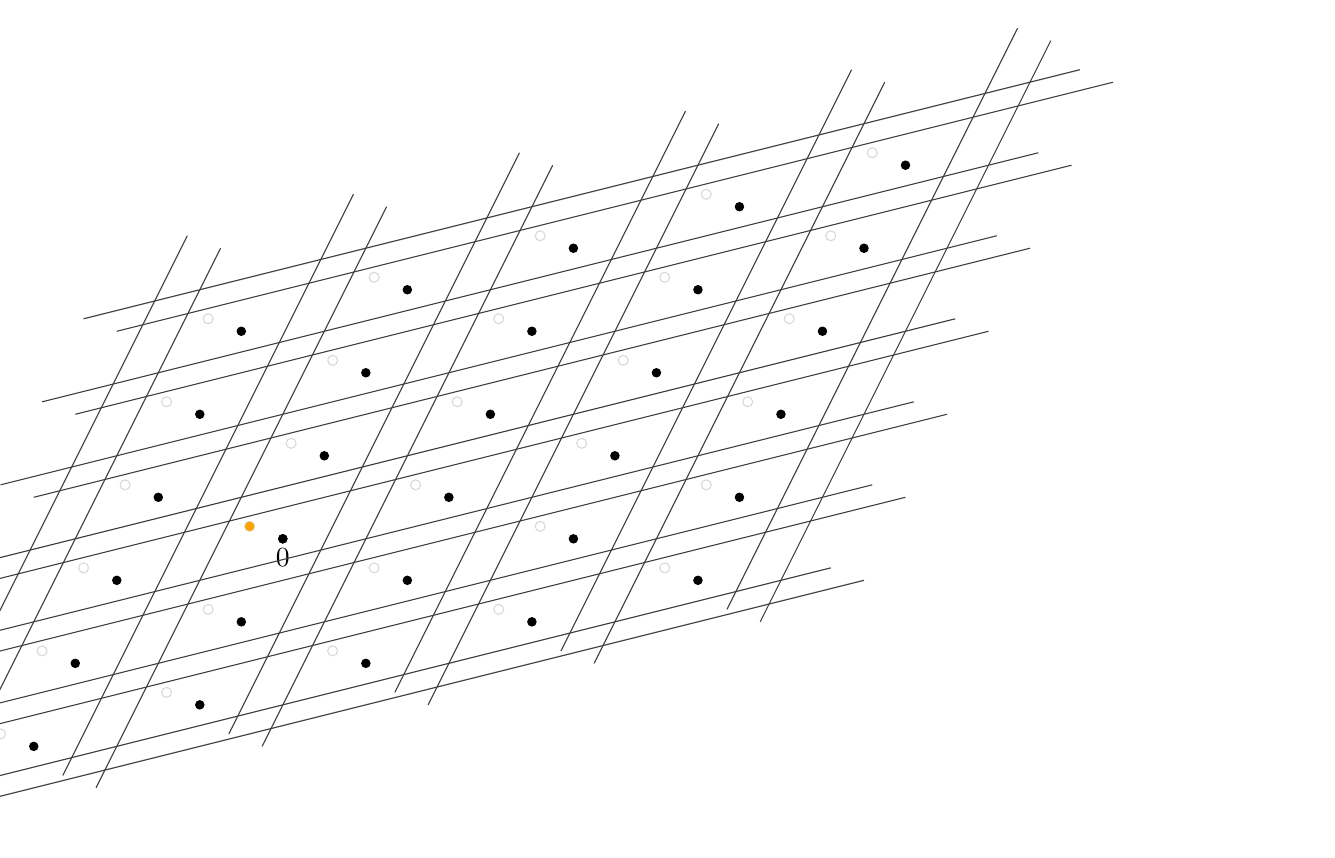
\begin{tikzpicture}%[show background grid]
\hspace{-70pt}
\vspace{-70pt}

\def\shiftx{-8pt}
\def\shifty{3pt}
\begin{scope}[scale=1.5]
\foreach \y in {-2,...,3}
{
	\foreach \x in {-1,...,3}
	{
		\filldraw(\x*40pt+\y*10pt, 10pt*\x+20pt*\y) circle (1.0pt);
		%\draw[fill=none, draw=gray] (\x*40pt+\y*10pt-15pt ,10pt*\x+20pt*\y-10pt) rectangle (\x*40pt+\y*10pt+15pt, 10pt*\x+20pt*\y+10pt);
	}
	
}
\foreach \x in {-1,...,4}
\draw[draw=CharCoalDark!80, shift={(-15pt,0pt)}] (\x*40pt-30pt, 10pt*\x-60pt) --  (\x*40pt+40pt, 10pt*\x+80pt);
\foreach \y in {-2,...,4}
\draw[draw=CharCoalDark!80, shift={(0pt,-10pt)}] (-80pt+\y*10pt, -20pt+20pt*\y) --  (160pt+\y*10pt, 40pt+20pt*\y);

\filldraw(0pt,0pt) circle (1.0pt) node[below]{ $0$};

\pause

\foreach \y in {-2,...,3}
{
	\foreach \x in {-1,...,3}
	{
		\filldraw[fill=white, draw=gray!30](\x*40pt+\y*10pt+\shiftx, 10pt*\x+20pt*\y+\shifty) circle (1.2pt);
	}
	
}
\foreach \x in {-1,...,4}
\draw[draw=CharCoalDark!80, shift={(-15pt,0pt)}] (\x*40pt-30pt+\shiftx, 10pt*\x-60pt+\shifty) --  (\x*40pt+40pt+\shiftx, 10pt*\x+80pt+\shifty);
\foreach \y in {-2,...,4}
\draw[draw=CharCoalDark!80, shift={(0pt,-10pt)}] (-80pt+\y*10pt+\shiftx, -20pt+20pt*\y+\shifty) --  (160pt+\y*10pt+\shiftx, 40pt+20pt*\y+\shifty);

\filldraw[color=Orange, draw=Orange](\shiftx,\shifty) circle (1.0pt) node[below]{ $\tvec$};




\end{scope}

\end{tikzpicture}
\end{frame}

\begin{frame}{Hardness of LWE}
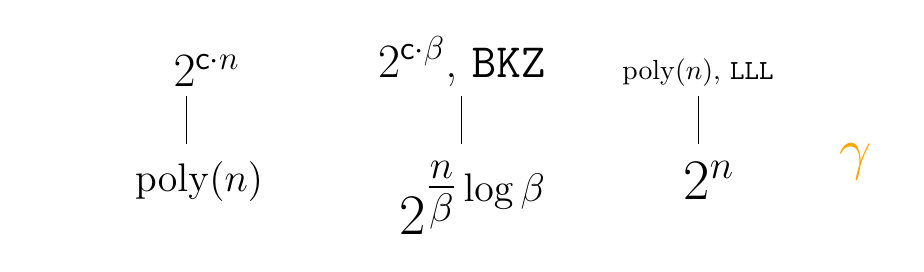
\begin{tikzpicture}
\draw[-stealth, white, thick] (0,0) -- (10.5, 0) node[font=\Large, below, yshift=-5pt]{\huge \color{Orange} $\mathbf{\gamma}$} node[above, yshift=4pt]{Time};

\draw[-] (2.0,-0.3) -- (2.0,0.3) node[above, xshift=10pt, align=center] {\LARGE $2^{\const  \cdot n}$ } node[below, yshift=-20pt, align=center, xshift=7pt] {\Large $\poly(n)$ };

\draw[-] (5.5,-0.3) -- (5.5,0.3) node[above] {\LARGE $ 2^{\const \cdot \beta}$, \texttt{BKZ}} node[below, yshift=-20pt, align=left, xshift=4pt] {\huge $2^{\tfrac{n}{\beta} \log \beta} $};

\draw[-] (8.5,-0.3) -- (8.5,0.3) node[above] {$\poly(n)$, \texttt{LLL}} node[below, yshift=-20pt, align=left, xshift=4pt] {\huge $2^{n}$};

\end{tikzpicture}
	\LARGE
	For LWE parameters $(n, m, q, \alpha)$, $\gamma = \frac{q^{1-n/m}}{\alpha q}$
	{
		
		%\begin{tcolorbox}[standard jigsaw, colback=CharCoalDark,
		%	opacityback=0.5,  colframe=Orange]
		{\color{Orange}
			\[
			T(\text{LWE}) = \exp\left(\const \cdot  \frac{\lg q}{\lg^2 \alpha} \lg\Big( \frac{n \lg q}{\lg^2 \alpha} \Big)  \cdot n\right),
			\]
		}
		%\end{tcolorbox}
	}

	where $\const$ is the constant in the exponent of SVP complexity, i.e., $T(\text{(SVP)})^{2^{\const \beta}}$.
	
	This complexity is obtained by solving for $\beta$
	\[
	2^{ \tfrac{m}{\beta} \log \beta} = \frac{q^{1-n/m}}{\alpha q}
	\]
	and choosing $m = \Omega(n)$ that minimizes the solution.
\end{frame}

\begin{frame}{Challenges}
\Large
\begin{center}
	\LARGE \color{Orange} Lattices
\end{center}
\begin{enumerate}
	\itemsep 7pt
	\item TU Darmstadt Challenges \url{https://www.latticechallenge.org/}
	\item Bochum challenges for Kyber \url{https://bochum-challeng.es/}
\end{enumerate}

\begin{center}
	\LARGE \color{Orange} Codes
\end{center}
\begin{enumerate}
	\itemsep 7pt
	\item Decoding (binary random, Goppa code, etc.) \url{https://decodingchallenge.org/}
	\item TII McEliece Challenges \url{https://www.herox.com/TIIMcElieceChallenges}
\end{enumerate}
\end{frame}

\begin{frame}{References}
	\begin{itemize}
		\setlength\itemsep{6pt}
		\item {\color{Orange} [BDGL16]}  A. Becker, L. Ducas, N. Gama, T. Laarhoven. New directions in nearest neighbor searching with applications to lattice sieving.
		\item {\color{Orange} [FP83]} U. Fincke and M. Pohst. A procedure for determining algebraic integers of given norm.
		\item {\color{Orange} [HS07]} Guillaume Hanrot and Damien Stehl{\'e}. Improved analysis of Kannan’s shortest lattice vector algorithm.
		\item {\color{Orange} [Kan83]} Ravi Kannan. Improved algorithms for integer programming and related lattice problems.
		\item {\color{Orange}[Kan87]} Ravi Kannan. Minkowski’s convex body theorem and integer programming. 
		\item {\color{Orange} [NV08]} P. Nguyen, T. Vidick. Sieve algorithms for the shortest vector problem are practical. 
		\item {\color{Orange}[S87]} Claus-Peter Schnorr. A hierarchy of polynomial time lattice basis reduction algorithms.

	\end{itemize}
\end{frame}



\end{document}